% !TeX program = xelatex
% !TeX encoding = UTF-8
% !TeX TXS-program:compile = txs:///xelatex | txs:///xelatex
\documentclass[aspectratio=169, table, 12pt]{beamer}

% Preamble bersama seluruh slide mata kuliah ini.
% Dipanggil dari slides/sessionXX/sessionXX.tex tepat sesudah baris
% \documentclass[aspectratio=169, table, 12pt]{beamer}
% Paket tambahan yang hanya dibutuhkan satu sesi ditulis di berkas sesi itu.

\usepackage{colortbl}
\usepackage{xcolor}
\usepackage{listings}
\usepackage{tabularx}
\usepackage{booktabs}
\usepackage{tikz}
\usepackage{pgfplots}
\usepackage{fontspec}
\usepackage[english,bahasai]{babel}
\pgfplotsset{compat=1.18}
\usetikzlibrary{arrows.meta, positioning, calc, fit, shapes.geometric,
  shapes.multipart, backgrounds, matrix, chains, trees}

\makeatletter
\def\input@path{{../theme/}}
\makeatother
\graphicspath{{../theme/}{../../figures/}}
% Stub symlink Windows memakai tema cadangan sampai aset institusi tersedia.
\IfFileExists{../theme/beamerthemePradita.sty}{%
  \usetheme{Pradita}
}{%
  \usetheme{Madrid}
  \setmainfont{TeX Gyre Heros}
  \setsansfont{TeX Gyre Heros}
  \setbeamertemplate{navigation symbols}{}
}

\definecolor{praditagreen}{RGB}{37, 113, 71}
\setbeamercolor{structure}{fg=praditagreen}
\setbeamercolor{palette primary}{bg=praditagreen,fg=white}
\setbeamercolor{palette secondary}{bg=praditagreen!80!black,fg=white}
\setbeamercolor{palette tertiary}{bg=praditagreen!60!black,fg=white}
\setbeamerfont{frametitle}{size=\large}
\setbeamertemplate{caption}[numbered]

% Ukuran header mengikuti teks agar judul panjang tidak menabrak logo.
\setbeamercolor{frametitle}{bg=white,fg=black}
\setbeamertemplate{frametitle}{%
  \begin{beamercolorbox}[wd=\paperwidth,sep=0.2cm]{frametitle}
    \begin{minipage}[c]{0.77\paperwidth}
      \raggedright\fontsize{16}{18}\selectfont\bfseries\insertframetitle
      \ifx\insertframesubtitle\empty\else
        \par\small\mdseries\insertframesubtitle
      \fi
    \end{minipage}\hfill
    \begin{minipage}[c]{0.15\paperwidth}
      \IfFileExists{../theme/classFiles/logo_universitas.png}{%
        
\includegraphics[width=\linewidth]{../theme/classFiles/logo_universitas.png}%
      }{}
    \end{minipage}
  \end{beamercolorbox}
}
\setbeamertemplate{footline}{%
  \ifnum\value{framenumber}>1
    \begin{beamercolorbox}[wd=\paperwidth,ht=0.35cm,dp=0.15cm,
      leftskip=0.3cm,rightskip=0.3cm]{palette primary}
      \footnotesize\bfseries\insertframenumber/\inserttotalframenumber
      \hfill IT40813
    \end{beamercolorbox}
  \fi
}
\DeclareRobustCommand{\berkas}[1]{\path{#1}}

% Tema membuat garis tabel berwarna putih. Dikembalikan agar tabel terbaca.
\arrayrulecolor{black}
\setlength{\arrayrulewidth}{0.5pt}

\lstdefinelanguage{yaml}{
  basicstyle=\ttfamily\scriptsize,
  keywordstyle=\color{blue}\bfseries,
  commentstyle=\color{gray}\itshape,
  stringstyle=\color{red},
  showstringspaces=false,
  breaklines=true,
  frame=lines,
  numbers=none,
  backgroundcolor=\color{lightgray!10},
  tabsize=2,
  morecomment=[l]{\#}
}

\lstdefinelanguage{json}{
  basicstyle=\ttfamily\scriptsize,
  stringstyle=\color{red},
  commentstyle=\color{gray},
  breaklines=true,
  showstringspaces=false,
  tabsize=2,
  numbers=none,
  frame=lines,
  backgroundcolor=\color{lightgray!10},
  string=[s]{"}{"}
}

\lstdefinelanguage{bash}{
  keywords={},
  basicstyle=\ttfamily\scriptsize,
  ndkeywords={docker, kubectl, helm, curl, git, terraform},
  ndkeywordstyle=\color{purple}\bfseries,
  sensitive=true,
  commentstyle=\color{gray},
  numbers=none,
  breaklines=true,
  frame=lines,
  backgroundcolor=\color{lightgray!10},
  tabsize=2,
  comment=[l]{\#},
  showstringspaces=false
}

\lstdefinelanguage{http}{
  keywords={GET, POST, PUT, PATCH, DELETE, HEAD, OPTIONS, HTTP},
  basicstyle=\ttfamily\scriptsize,
  keywordstyle=\color{blue}\bfseries,
  sensitive=true,
  numbers=none,
  breaklines=true,
  frame=lines,
  backgroundcolor=\color{lightgray!10},
  tabsize=2,
  showstringspaces=false
}

\subtitle{IT40813 · IT Governance, Risk \& Compliance}
\author{\textbf{Alfa Yohannis}}


% Sampul membatasi judul di panel putih tema rujukan Pradita.
\setbeamertemplate{title page}{%
  \begin{tikzpicture}[remember picture,overlay]
    \node[anchor=north west,inner sep=0pt,text width=8.8cm]
      at ([xshift=1cm,yshift=-3.15cm]current page.north west) {%
        {\small\insertsubtitle\par}\vspace{0.25cm}
        \resizebox{8.8cm}{!}{\begin{minipage}{12cm}
          \raggedright\color{praditagreen}\bfseries\inserttitle
        \end{minipage}}
      };
    \node[anchor=south west,inner sep=0pt]
      at ([xshift=1cm,yshift=1.65cm]current page.south west)
      {\small\insertdate};
    \node[anchor=west,inner sep=0pt,text=white]
      at ([xshift=0.8cm,yshift=0.75cm]current page.south west)
      {\small\insertauthor};
  \end{tikzpicture}
}


\title{\Huge Audit TI\\ \vspace{10pt} dan Asurans}
\date{Pertemuan 12}

\begin{document}

\frame{\titlepage}

\begin{frame}
  \frametitle{Isi Pertemuan}
  \vspace{14pt}
  \begin{columns}[t]
    \column{0.5\textwidth}
    {\small\tableofcontents[sections={1-5}]}

    \column{0.5\textwidth}
    {\small\tableofcontents[sections={6-10}]}
  \end{columns}
\end{frame}

\begin{frame}{\hfill}
  \centering
  \Huge{\textbf{Unit TI melapor 108 dari 108.\\Mengapa audit tetap\\menemukan masalah?}}
\end{frame}

\section{Tujuan dan Konteks}

\begin{frame}{{\Large Tujuan Pembelajaran}}
  \vspace{10pt}
  \begin{itemize}
    \item Menjelaskan pembagian peran dalam Three Lines Model dan posisi audit internal yang
          independen.
    \item Menyusun rencana asurans berbasis risiko untuk program transformasi digital.
    \item Menguji rancangan dan efektivitas satu kontrol dengan bukti yang memadai.
  \end{itemize}
\end{frame}

\begin{frame}{{\Large Masalah: Dua Laporan, Dua Penyebut}}
  \vspace{6pt}
  \small
  \begin{itemize}
    \item Misalkan unit TI melapor: 108 dari 108 akun sudah ditinjau.
    \item Audit internal memeriksa 30 dari 120 akun: 6 akun masih aktif setelah penugasan berakhir.
    \item Keduanya dapat benar. Daftar unit TI hanya memuat 108 akun, sehingga 12 akun luput.
    \item Dengan penyebut yang benar, cakupannya 90 persen, bukan 100 persen.
    \item Hasil kerja: rencana asurans dua tahun dan contoh pengujian satu kontrol untuk C4.
  \end{itemize}
\end{frame}

\begin{frame}{{\Large Diagram Konsep Bab 12}}
  \centering
  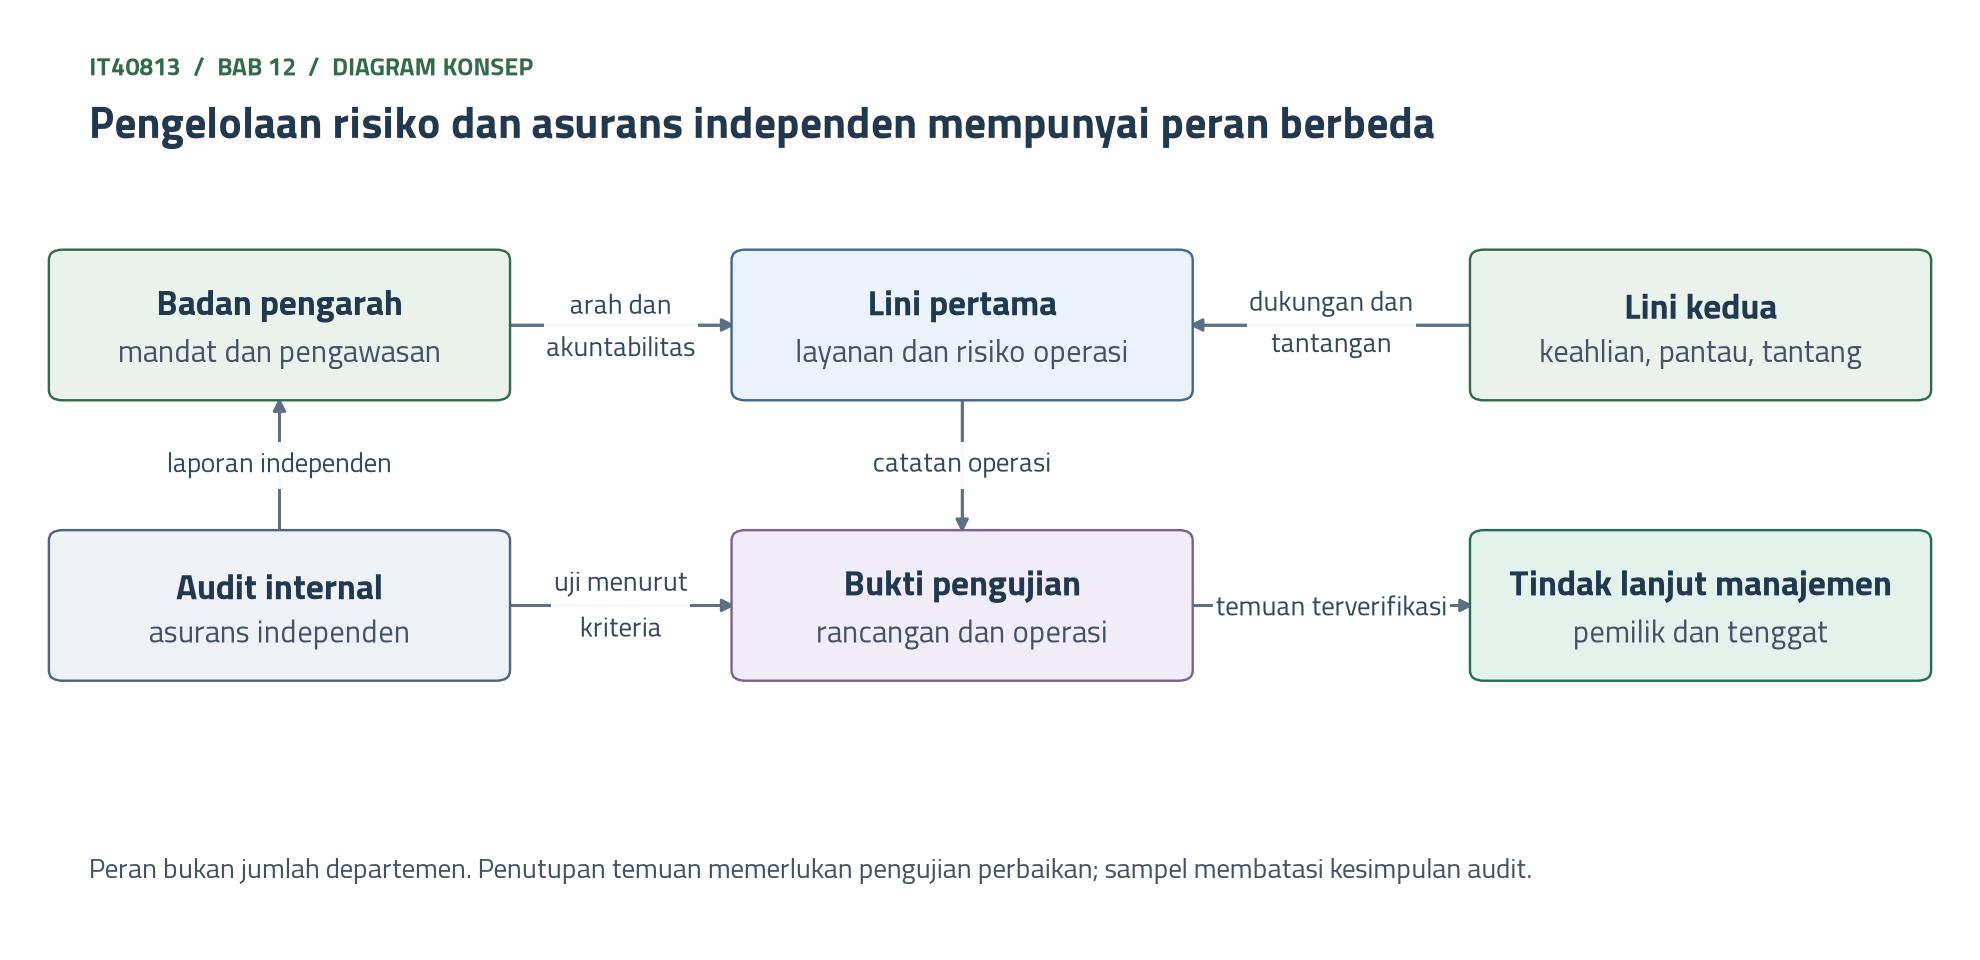
\includegraphics[width=0.96\textwidth,height=0.77\textheight,keepaspectratio]{../../figures/ch12-diagram-konsep.png}
  \label{fig:session12-ilustrasi-bab}
\end{frame}

\section{Konsep Asurans}

\begin{frame}{{\Large Asurans: Keyakinan yang Punya Batas}}
  \vspace{4pt}
  \scriptsize
  \begin{tabularx}{\textwidth}{|>{\raggedright\arraybackslash}p{0.17\textwidth}|>{\raggedright\arraybackslash}X|>{\raggedright\arraybackslash}X|}
    \hline
    \textbf{Pertanyaan} & \textbf{Laporan unit TI} & \textbf{Pengujian audit internal} \\ \hline
    Kriteria & Akun pada daftar sudah ditinjau & Dicabut paling lambat 1 hari kerja setelah
    penugasan berakhir \\ \hline
    Populasi & 108 akun pada daftar peninjau & 120 akun pada daftar penugasan \\ \hline
    Periode & Satu bulan terakhir, tanpa tanggal & Tanggal acuan 31 Maret 2026 \\ \hline
    Metode & Pernyataan pelaksana & Pencocokan dokumen dan 30 akun sampel \\ \hline
    Pengecualian & Tidak disebut & Sampel satu lokasi; 4 rumah sakit lain belum punya bukti \\
    \hline
  \end{tabularx}

  \vspace{8pt}
  \small Analogi pemeriksaan kendaraan: uji rem pada satu tanggal memberi bukti kondisi itu, bukan
  jaminan tidak akan pernah terjadi kecelakaan.
\end{frame}

\begin{frame}{{\Large Asurans dan Konsultasi}}
  \vspace{4pt}
  \scriptsize
  \begin{tabularx}{\textwidth}{|>{\raggedright\arraybackslash}p{0.2\textwidth}|>{\raggedright\arraybackslash}X|>{\raggedright\arraybackslash}X|}
    \hline
    \textbf{Aspek} & \textbf{Asurans} & \textbf{Konsultasi} \\ \hline
    Tujuan & Menilai terhadap kriteria & Membantu perbaikan \\ \hline
    Kriteria & Wajib ditetapkan & Dapat tidak diperlukan, sesuai kesepakatan \\ \hline
    Keluaran & Kesimpulan dan temuan & Saran dan pilihan \\ \hline
    Tanggung jawab kontrol & Tetap pada manajemen & Tetap pada manajemen \\ \hline
    Pengaman & Penilai tidak menjalankan proses yang dinilai & Peran jelas; keputusan pada
    manajemen; badan pengarah diberi tahu \\ \hline
  \end{tabularx}

  \vspace{8pt}
  \small Analogi guru les dan penguji: satu orang boleh memegang keduanya pada waktu berbeda, tetapi
  tidak menilai jawaban yang ia diktekan sendiri.
\end{frame}

\begin{frame}{{\Large Dua Contoh Pemisahan}}
  \vspace{6pt}
  \small
  \begin{itemize}
    \item Misalkan audit internal memberi saran 40 jam untuk KB-09 pada Tahun 1.
    \item Pemilik KB-09 tetap direktur pelayanan. Audit AI pada Tahun 2 dipimpin auditor lain.
    \item IIA: masa paling sedikit 12 bulan biasanya memadai antara tanggung jawab atas proses dan
          pemberian asurans.
    \item Misalkan petugas operasi TI menjalankan AC-01 sampai 31 Maret 2026, lalu pindah ke audit.
    \item Dengan acuan itu, ia sebaiknya tidak menguji AC-01 sebelum 1 April 2027.
  \end{itemize}
\end{frame}

\section{Three Lines Model}

\begin{frame}{{\Large Three Lines Model pada AC-01}}
  \vspace{2pt}
  \begin{center}
    \resizebox{0.86\textwidth}{!}{\begin{tikzpicture}[
  font=\scriptsize,
  kotak/.style={draw, rounded corners, align=center, text width=2.85cm, minimum height=1.7cm},
  panah/.style={-{Stealth[length=2mm]}, thick}]
  \node[draw, rounded corners, align=center, text width=10.3cm, minimum height=0.95cm,
    fill=praditagreen!15] (bp) at (0,0)
    {\textbf{Badan pengarah}\\Dewan komisaris mengawasi, direksi memutuskan sesuai kewenangan};
  \node[kotak, fill=blue!8] (l1) at (-3.65,-2.45)
    {\textbf{Lini pertama}\\pemilik Medikara+, kepala operasi TI\\
    {\tiny\mdseries menjalankan AC-01, 60 catatan per tahun}};
  \node[kotak, fill=blue!8] (l2) at (0,-2.45)
    {\textbf{Lini kedua}\\CISO, kepala risiko\\
    {\tiny\mdseries memantau dan menantang cakupan 120 akun}};
  \node[kotak, fill=orange!12] (l3) at (3.65,-2.45)
    {\textbf{Lini ketiga}\\audit internal\\
    {\tiny\mdseries menguji secara independen, termasuk lini kedua}};
  \node[draw, dashed, rounded corners, align=center, text width=10.3cm, minimum height=0.8cm,
    fill=gray!10] (luar) at (0,-4.55)
    {\textbf{Pihak luar, bukan bagian dari tiga lini}: auditor eksternal, regulator, laporan SOC 2};
  \draw[panah] (bp.south -| l1) -- (l1) node[midway, left] {{\tiny\mdseries arah}};
  \draw[panah] (l2) -- (l1);
  \draw[panah] (l3.north) -- (bp.south -| l3) node[midway, right] {{\tiny\mdseries fungsional}};
  \draw[panah, dashed] (luar.north -| l3) -- (l3) node[midway, right] {{\tiny\mdseries koordinasi}};
  \draw[panah, dashed] (luar.north -| l1) -- (l1) node[midway, left] {{\tiny\mdseries laporan}};
\end{tikzpicture}
}
  \end{center}
\end{frame}

\begin{frame}{{\Large Kekuatan dan Batas Tiap Peran}}
  \vspace{4pt}
  \scriptsize
  \begin{tabularx}{\textwidth}{|>{\raggedright\arraybackslash}p{0.15\textwidth}|>{\raggedright\arraybackslash}p{0.25\textwidth}|>{\raggedright\arraybackslash}X|>{\raggedright\arraybackslash}X|}
    \hline
    \textbf{Peran} & \textbf{Contoh pemilik} & \textbf{Tanggung jawab} & \textbf{Batas} \\ \hline
    Badan pengarah & Dewan komisaris dan direksi sesuai kewenangan & Menetapkan arah, mengawasi &
    Bergantung pada informasi andal \\ \hline
    Lini pertama & Pemilik Medikara+, kepala operasi TI, pemilik SIMRS & Menjalankan AC-01 & Dapat
    meremehkan kelemahan kontrolnya \\ \hline
    Lini kedua & CISO, kepala risiko, petugas pelindungan data & Memantau dan menantang & Kadang
    terganggu karena melapor lewat manajemen \\ \hline
    Lini ketiga & Audit internal & Menguji secara independen & Berkala dan berbasis risiko \\ \hline
  \end{tabularx}

  \vspace{8pt}
  \small Peran, bukan jumlah departemen. Pengalihan pekerjaan ke vendor tidak mengubah
  akuntabilitas.
\end{frame}

\begin{frame}{{\Large Independensi: Lima Unsur}}
  \vspace{4pt}
  \scriptsize
  \begin{tabularx}{\textwidth}{|>{\raggedright\arraybackslash}p{0.27\textwidth}|>{\raggedright\arraybackslash}X|>{\raggedright\arraybackslash}X|}
    \hline
    \textbf{Unsur} & \textbf{Bukti yang diperiksa} & \textbf{Tanda masalah} \\ \hline
    Jalur pelaporan dan wewenang & Piagam audit; laporan ke komite audit & Laporan harus melewati
    kepala TI \\ \hline
    Otonomi ruang lingkup & Rencana disetujui dewan komisaris & Area AC-01 dicoret pihak yang
    diperiksa \\ \hline
    Akses tanpa batas & Hak meminta daftar penugasan langsung & Daftar hanya datang dari operasi TI
    \\ \hline
    Kendali sumber daya & Jam dan keahlian pada rencana & Jam dipotong tanpa dilaporkan \\ \hline
    Perlindungan dari tekanan & Catatan perubahan laporan audit & Temuan diubah atas permintaan
    pemilik proses \\ \hline
  \end{tabularx}

  \vspace{8pt}
  \small Unit risiko melapor kepada direktur TI? Jabatan atasan saja belum membuktikan pelanggaran.
  Periksa mandat, akses, dan pengamannya.
\end{frame}

\section{Standar Profesi}

\begin{frame}{{\Large Global Internal Audit Standards}}
  \vspace{2pt}
  \scriptsize
  \begin{tabularx}{\textwidth}{|>{\raggedright\arraybackslash}p{0.09\textwidth}|>{\raggedright\arraybackslash}X|>{\raggedright\arraybackslash}p{0.33\textwidth}|}
    \hline
    \textbf{Standar} & \textbf{Ketentuan ringkas} & \textbf{Bukti contoh} \\ \hline
    7.1 & Independensi dikonfirmasi paling sedikit setahun sekali & Pernyataan tahunan \\ \hline
    8.4 & Penilaian mutu eksternal paling sedikit sekali dalam lima tahun & Rencana penilaian \\
    \hline
    9.4 & Rencana audit berdasar penilaian risiko terdokumentasi, paling sedikit setahun sekali &
    Semesta audit \\ \hline
    9.5 & Koordinasi; dasar kepercayaan didokumentasikan & Peta asurans \\ \hline
    14.1 & Informasi relevan, andal, dan cukup & Kertas kerja 30 akun \\ \hline
    15.2 & Pelaksanaan rekomendasi dikonfirmasi dan dilacak & Status penutupan TA-01 \\ \hline
  \end{tabularx}

  \vspace{6pt}
  \small Berlaku sejak 9 Januari 2025: 5 domain, 15 prinsip, 52 standar. Ringkasan ini bukan
  terjemahan resmi.
\end{frame}

\begin{frame}{{\Large ITAF dan Acuan Terbuka}}
  \vspace{6pt}
  \small
  \begin{itemize}
    \item ITAF edisi kelima adalah kerangka ISACA untuk audit dan asurans TI. Naskahnya berbayar.
    \item FISCAM revisi 2026 terbuka dan menjelaskan cara menguji kontrol sistem informasi.
    \item Government Auditing Standards 2024 terbuka dan menjelaskan unsur temuan.
    \item Keduanya ditulis untuk audit pemerintah Amerika Serikat, sehingga menjadi contoh metode.
    \item Analogi klinik kecil: ukuran mengubah cara dokumentasi, bukan kebutuhan akan catatan.
  \end{itemize}
\end{frame}

\section{Perencanaan Berbasis Risiko}

\begin{frame}{{\Large Siklus Asurans}}
  \vspace{8pt}
  \begin{center}
    \resizebox{0.95\textwidth}{!}{\begin{tikzpicture}[
  font=\scriptsize,
  kotak/.style={draw, rounded corners, align=center, text width=3.15cm, minimum height=1.2cm},
  panah/.style={-{Stealth[length=2mm]}, thick}]
  \node[kotak, fill=praditagreen!15] (a) at (0,0)
    {\textbf{Mandat dan risiko}\\{\tiny\mdseries register R-01 sampai R-12}};
  \node[kotak, fill=blue!8] (b) at (4,0)
    {\textbf{Rencana asurans}\\{\tiny\mdseries area, waktu, dan jam}};
  \node[kotak, fill=blue!8] (c) at (8,0)
    {\textbf{Program audit}\\{\tiny\mdseries kriteria, populasi, prosedur}};
  \node[kotak, fill=orange!12] (d) at (8,-2)
    {\textbf{Bukti pengujian}\\{\tiny\mdseries rancangan dan operasi}};
  \node[kotak, fill=orange!12] (e) at (4,-2)
    {\textbf{Temuan}\\{\tiny\mdseries kondisi, kriteria, sebab, akibat}};
  \node[kotak, fill=green!10] (f) at (0,-2)
    {\textbf{Tindak lanjut terverifikasi}\\{\tiny\mdseries pemilik, tenggat, uji ulang}};
  \draw[panah] (a) -- (b);
  \draw[panah] (b) -- (c);
  \draw[panah] (c) -- (d);
  \draw[panah] (d) -- (e);
  \draw[panah] (e) -- (f);
  \draw[panah] (f) -- (a) node[midway, left, align=right]
    {{\tiny\mdseries risiko}\\{\tiny\mdseries dinilai ulang}};
\end{tikzpicture}
}
  \end{center}
  \vspace{4pt}
  \small Analogi pemeriksaan rumah: retakan struktur dan lampu hias mati tidak diperiksa dengan
  prioritas sama.
\end{frame}

\begin{frame}{{\Large Semesta Audit dan Skor Prioritas (Misalkan)}}
  \vspace{0pt}
  \scriptsize
  \begin{tabularx}{\textwidth}{|>{\raggedright\arraybackslash}X|c|c|c|c|c|c|c|}
    \hline
    \textbf{Area} & \textbf{Risiko} & \textbf{Skor} & \textbf{Ubah} & \textbf{Wajib} &
    \textbf{Lain} & \textbf{Prioritas} & \textbf{Jam} \\ \hline
    Akses vendor AC-01 & R-01 & 12 & 3 & 5 & 1 & 19 & 600 \\ \hline
    AI klinis AI-01, AI-02 & R-11 & 12 & 5 & 3 & 1 & 19 & 480 \\ \hline
    Pemulihan DSS04 & R-05 & 10 & 5 & 2 & 1 & 16 & 480 \\ \hline
    Jejak aktivitas KB-06 & R-02 & 12 & 3 & 3 & 2 & 16 & 240 \\ \hline
    Privasi dan retensi & R-09 & 9 & 3 & 5 & 2 & 15 & 200 \\ \hline
    Insiden dan pemberitahuan & R-12 & 8 & 3 & 5 & 2 & 14 & 240 \\ \hline
    Vendor inti dan cloud & R-08 & 8 & 5 & 3 & 3 & 13 & 320 \\ \hline
    Integrasi BPJS Kesehatan & R-03 & 9 & 3 & 2 & 1 & 13 & 200 \\ \hline
    Laporan spreadsheet & R-04 & 12 & 1 & 1 & 4 & 10 & 240 \\ \hline
    Rilis Medikara+ & R-07 & 9 & 2 & 1 & 2 & 10 & 240 \\ \hline
    \textbf{Jumlah} & & & & & & & \textbf{3.240} \\ \hline
  \end{tabularx}

  \vspace{4pt}
  \scriptsize Prioritas = skor risiko + perubahan + kewajiban $-$ asurans lain. Rumus pembelajaran,
  bukan ketentuan standar.
\end{frame}

\begin{frame}{{\Large Kapasitas Membatasi Pilihan}}
  \vspace{6pt}
  \small
  \begin{itemize}
    \item 1 auditor TI 1.200 jam dan 1 auditor umum 600 jam: 1.800 jam per tahun, 3.600 jam dua
          tahun.
    \item Cadangan 20 persen mengambil 720 jam, sehingga jam terencana 2.880.
    \item Kebutuhan 3.240 jam. Dua area berprioritas terendah, 480 jam, ditunda. Sisa 120 jam.
    \item Celah cakupan dilaporkan kepada dewan komisaris. R-04 tetap berharapan kerugian Rp30 juta.
    \item Skor tidak mekanis: pemulihan harus sebelum migrasi, dan cedera berat memakai cadangan.
  \end{itemize}
\end{frame}

\begin{frame}{{\Large Rencana Asurans Dua Tahun (Misalkan)}}
  \vspace{0pt}
  \scriptsize
  \begin{tabularx}{\textwidth}{|>{\raggedright\arraybackslash}p{0.17\textwidth}|>{\raggedright\arraybackslash}X|>{\raggedright\arraybackslash}p{0.07\textwidth}|>{\raggedright\arraybackslash}X|}
    \hline
    \textbf{Waktu} & \textbf{Area} & \textbf{Jam} & \textbf{Keputusan yang didukung} \\ \hline
    Tahun 1 awal & Akses vendor AC-01 & 600 & Kesiapan perluasan mitra \\ \hline
    Tahun 1 akhir & Pemulihan DSS04 & 480 & Kesiapan kelangsungan \\ \hline
    Tahun 1 akhir & Insiden dan pemberitahuan & 240 & Kesiapan pemberitahuan \\ \hline
    Sepanjang Tahun 1 & Saran KB-09, laporan pihak luar & 120 & Rancangan kebijakan AI \\ \hline
    Tahun 2 & AI klinis AI-01, AI-02 & 480 & Batas perluasan AI \\ \hline
    Tahun 2 & Jejak aktivitas KB-06 & 240 & Keandalan penelusuran \\ \hline
    Tahun 2 & Privasi dan retensi & 200 & Batas pemakaian data \\ \hline
    Tahun 2 & Vendor inti dan cloud & 320 & Perpanjangan kontrak \\ \hline
    Tahun 2 & Integrasi BPJS Kesehatan & 200 & Kelangsungan pendaftaran \\ \hline
  \end{tabularx}

  \vspace{4pt}
  \scriptsize Tiap tahun 1.440 jam. Bila kapasitas dipangkas menjadi 1.200 jam, audit pemulihan
  tidak muat, dan pemangkasan itu dilaporkan ke komite audit.
\end{frame}

\begin{frame}{{\Large Peta Asurans (Misalkan)}}
  \vspace{0pt}
  \scriptsize
  \begin{tabularx}{\textwidth}{|>{\raggedright\arraybackslash}p{0.17\textwidth}|>{\raggedright\arraybackslash}X|>{\raggedright\arraybackslash}X|>{\raggedright\arraybackslash}p{0.09\textwidth}|>{\raggedright\arraybackslash}p{0.18\textwidth}|}
    \hline
    \textbf{Area} & \textbf{Lini pertama} & \textbf{Lini kedua} & \textbf{Audit} &
    \textbf{Pihak luar} \\ \hline
    Akses vendor AC-01 & 60 catatan per tahun & CISO memantau 120 akun & Tahun 1 & SOC 2, sisi
    penyedia \\ \hline
    Pemulihan DSS04 & 144 uji per tahun & Kepala risiko meninjau hasil & Tahun 1 & Tidak ada \\
    \hline
    Insiden & Prosedur KB-07 & Petugas pelindungan data, 2 latihan & Tahun 1 & Tidak ada \\ \hline
    Jejak aktivitas & Tinjauan catatan aktivitas & CISO, 247 dari 260 tinjauan & Tahun 2 & Tidak
    ada \\ \hline
    AI klinis & Uji AI-01, AI-02 & Kepala risiko, petugas pelindungan data & Tahun 2 & Tidak ada \\
    \hline
    Vendor dan cloud & Pengelola vendor & Kepala risiko, register pemasok & Tahun 2 & SOC 2 Type 2,
    sertifikat \\ \hline
    Laporan spreadsheet & Rekonsiliasi manual & Kepala risiko & Ditunda & Audit keuangan saja \\
    \hline
  \end{tabularx}

  \vspace{4pt}
  \scriptsize Bab 1: 276 permintaan menjadi 92 menghemat 368 jam, atau Rp22,08 juta per tahun. Audit
  internal dapat memilih tidak mengandalkan pekerjaan yang mutunya kurang.
\end{frame}

\section{Pengujian Kontrol}

\begin{frame}{{\Large Uji Rancangan dan Uji Efektivitas}}
  \vspace{0pt}
  \begin{center}
    \resizebox{0.8\textwidth}{!}{\begin{tikzpicture}[
  font=\scriptsize,
  sel/.style={draw, rounded corners, align=left, text width=4.55cm, minimum height=2cm},
  judul/.style={font=\footnotesize\bfseries, align=center}]
  \node[sel, fill=green!10] (a) at (0,0)
    {\textbf{Rancangan memadai, operasi berjalan}\\Kesimpulan efektif untuk lingkup itu.
    \\{\tiny\mdseries Sasaran: 120 dari 120 akun, 60 dari 60 catatan}};
  \node[sel, fill=orange!12] (b) at (5.05,0)
    {\textbf{Rancangan memadai, operasi tidak berjalan}\\Perbaiki pelaksanaan, bukan kebijakan.
    \\{\tiny\mdseries Contoh: 12 dari 60 catatan tersedia}};
  \node[sel, fill=orange!12] (c) at (0,-2.2)
    {\textbf{Rancangan lemah, operasi berjalan}\\Kontrol rajin dijalankan, tetapi meleset.
    \\{\tiny\mdseries Contoh: 108 dari 108 ditinjau, 12 akun luput}};
  \node[sel, fill=red!22] (d) at (5.05,-2.2)
    {\textbf{Rancangan lemah, operasi tidak berjalan}\\Risiko belum ditangani.
    \\{\tiny\mdseries Contoh: rumah sakit tanpa peninjauan dan tanpa daftar}};
  \node[judul] at (0,1.3) {Operasi berjalan};
  \node[judul] at (5.05,1.3) {Operasi tidak berjalan};
  \node[judul, rotate=90] at (-2.95,0) {Rancangan\\memadai};
  \node[judul, rotate=90] at (-2.95,-2.2) {Rancangan\\lemah};
\end{tikzpicture}
}
  \end{center}
  \vspace{-4pt}
  \scriptsize Analogi pintu: rancangan kunci dapat memadai, tetapi bukti pintu dikunci setiap malam
  memerlukan catatan pelaksanaan.
\end{frame}

\begin{frame}{{\Large Program Audit AC-01 (Misalkan)}}
  \vspace{2pt}
  \scriptsize
  \begin{tabularx}{\textwidth}{|>{\raggedright\arraybackslash}X|>{\raggedright\arraybackslash}p{0.14\textwidth}|>{\raggedright\arraybackslash}X|>{\raggedright\arraybackslash}p{0.2\textwidth}|}
    \hline
    \textbf{Pertanyaan} & \textbf{Jenis uji} & \textbf{Bukti} & \textbf{Hasil contoh} \\ \hline
    Siapa boleh menyetujui dan menjalankan? & Rancangan & Prosedur KB-03, pemisahan tugas & Ada
    pemisahan tugas \\ \hline
    Apakah daftar peninjau lengkap? & Rancangan & Daftar peninjau, daftar penugasan & 108 dari 120
    akun \\ \hline
    Apakah peninjauan bulanan di 5 rumah sakit? & Operasi & Catatan per lokasi & 12 dari 60
    catatan \\ \hline
    Apakah akun dicabut paling lambat 1 hari kerja? & Operasi & Sampel 30 akun, tiket & 24 sesuai, 6
    menyimpang \\ \hline
    Apakah pengecualian ditutup? & Tindak lanjut & Tiket, verifikasi ulang & 24 dicabut, lalu 9, 5,
    2 \\ \hline
  \end{tabularx}
\end{frame}

\begin{frame}{{\Large Kriteria Ditetapkan Sebelum Data Dibuka}}
  \vspace{6pt}
  \small
  \begin{itemize}
    \item Data latihan: 8 akun sintetis, 30 Oktober 2026. Satu tidak aktif dikeluarkan, jadi 7
          aktif.
    \item USR002 tanpa pemilik, USR003 akun bersama dan terlambat, USR005 terlambat.
    \item Hasilnya 3 akun, 4 indikasi. Tinjauan tepat waktu 5 dari 7, atau 71,43 persen.
    \item Batas 90 hari hanya aturan skenario. Dengan 31 hari, hasilnya 3 dari 7, atau 42,86 persen.
    \item Indikasi memicu pemeriksaan lanjutan, bukan vonis penyalahgunaan.
  \end{itemize}
\end{frame}

\section{Bukti dan Sampel}

\begin{frame}{{\Large Empat Jenis Uji pada AC-01}}
  \vspace{4pt}
  \scriptsize
  \begin{tabularx}{\textwidth}{|>{\raggedright\arraybackslash}p{0.17\textwidth}|>{\raggedright\arraybackslash}X|>{\raggedright\arraybackslash}X|}
    \hline
    \textbf{Jenis} & \textbf{Cara pada AC-01} & \textbf{Batasnya} \\ \hline
    Bertanya & Kepala operasi TI menjelaskan cara peninjauan & Tidak cukup bila berdiri sendiri \\
    \hline
    Mengamati & Auditor mendampingi peninjauan satu rumah sakit & Tidak membuktikan waktu lain \\
    \hline
    Memeriksa dokumen & Catatan bulanan dan tiket pencabutan & Dokumen prosedur hanya membuktikan
    rancangan \\ \hline
    Mengulang & Auditor mencocokkan akun dengan daftar penugasan & Perlu akses dan pemeriksaan
    kelengkapan data \\ \hline
  \end{tabularx}

  \vspace{8pt}
  \small Bab 10: 29 dari 36 uji lulus, atau 80,6 persen. Pada 5 rumah sakit hanya 3 yang lulus, atau
  60 persen. Angka gabungan menyamarkan lokasi.
\end{frame}

\begin{frame}{{\Large Populasi Lebih Dahulu}}
  \vspace{4pt}
  \begin{center}
    \resizebox{0.9\textwidth}{!}{\begin{tikzpicture}[
  font=\scriptsize,
  kotak/.style={draw, rounded corners, align=center, text width=2.9cm, minimum height=1.05cm},
  panah/.style={-{Stealth[length=2mm]}, thick}]
  \node[kotak, fill=praditagreen!15] (pop) at (0,0)
    {\textbf{Daftar penugasan}\\120 akun vendor\\{\tiny\mdseries sumber di luar sistem yang diperiksa}};
  \node[kotak, fill=blue!8] (dft) at (4.2,1.5)
    {\textbf{Daftar peninjau}\\108 akun\\{\tiny\mdseries ditarik dari sistem yang diperiksa}};
  \node[kotak, fill=blue!8] (smp) at (4.2,0)
    {\textbf{Sampel audit}\\30 akun, satu lokasi};
  \node[kotak, fill=blue!8] (pny) at (4.2,-1.5)
    {\textbf{Peninjauan penuh}\\120 akun, bulan berikutnya};
  \node[kotak, fill=red!22] (luput) at (8.4,1.5)
    {\textbf{12 akun luput}\\{\tiny\mdseries cakupan 108 dari 120, atau 90 persen}};
  \node[kotak, fill=orange!12] (hsl) at (8.4,0)
    {\textbf{24 akun sesuai, 6 menyimpang}\\{\tiny\mdseries 80 dan 20 persen dari 30 akun}};
  \node[kotak, fill=orange!12] (cbt) at (8.4,-1.5)
    {\textbf{24 akun dicabut}\\{\tiny\mdseries 20 persen dari 120 akun}};
  \draw[panah] (pop.east) -- ++(0.35,0) |- (dft.west);
  \draw[panah] (pop) -- (smp);
  \draw[panah] (pop.east) -- ++(0.35,0) |- (pny.west);
  \draw[panah] (dft) -- (luput);
  \draw[panah] (smp) -- (hsl);
  \draw[panah] (pny) -- (cbt);
\end{tikzpicture}
}
  \end{center}
  \vspace{2pt}
  \scriptsize Dua angka 24: 24 dari 30 akun sampel sesuai (80 persen), dan 24 dari 120 akun dicabut
  (20 persen). Yang pertama menghitung akun sesuai, yang kedua akun bermasalah.
\end{frame}

\begin{frame}{{\Large Sampel Statistik dan Sampel Terarah}}
  \vspace{6pt}
  \small
  \begin{itemize}
    \item Sampel statistik dipilih acak dan dapat diproyeksikan. Sampel terarah tidak dimaksudkan
          begitu.
    \item Sampel 30 akun Bab 4 hanya mewakili satu lokasi, sehingga 20 persen tidak diproyeksikan.
    \item Analogi sayur: satu sendok dari permukaan panci hanya menjelaskan permukaannya.
    \item Misalkan audit ulang bertingkat: 40, 24, 20, 20, 16 akun menjadi sampel 10, 6, 5, 5, 4.
    \item Sampel dari daftar 108 tidak mungkin menyentuh 12 akun yang luput.
  \end{itemize}
\end{frame}

\begin{frame}{{\Large Apa yang Dapat Dikatakan Sampel Acak?}}
  \vspace{2pt}
  \scriptsize
  \begin{tabularx}{\textwidth}{|>{\raggedright\arraybackslash}X|c|c|c|}
    \hline
    \textbf{Hasil pada sampel 30} & \textbf{Perkiraan titik} & \textbf{Batas bawah} & \textbf{Batas
    atas} \\ \hline
    6 dari 30 menyimpang & 24 akun & 13 akun & 40 akun \\ \hline
    2 dari 30 menyimpang & 8 akun & 2 akun & 21 akun \\ \hline
    0 dari 30 menyimpang & 0 akun & 0 akun & 9 akun \\ \hline
  \end{tabularx}

  \vspace{6pt}
  \begin{tabularx}{\textwidth}{|>{\raggedright\arraybackslash}X|c|c|}
    \hline
    \textbf{Akun bermasalah pada populasi} & \textbf{Peluang tertangkap sampel 30} &
    \textbf{Sampel minimal 95 persen} \\ \hline
    12 akun & 97,40 persen & 26 akun \\ \hline
    2 akun & 43,91 persen & 93 akun \\ \hline
    1 akun & 25,00 persen & 114 akun \\ \hline
  \end{tabularx}

  \vspace{6pt}
  \scriptsize Populasi 120 akun, sebaran hipergeometrik, keyakinan 95 persen satu sisi.
\end{frame}

\begin{frame}{{\Large Toleransi Nol Menuntut Uji Seluruh Populasi}}
  \vspace{6pt}
  \small
  \begin{itemize}
    \item Hasil 30 dari 30 masih menyisakan kemungkinan sampai 9 akun bermasalah.
    \item \textit{Risk appetite} nol akun tanpa pemilik karena itu diuji pada 120 dari 120 akun.
    \item Manual 20 menit per akun: 40 jam atau Rp2,4 juta. Dengan skrip: 12 jam atau Rp720 ribu.
    \item Harapan kerugian R-01 Rp100 juta per tahun. Biaya bukan alasan untuk tidak menguji semua.
    \item Sampel tetap berguna untuk keaslian persetujuan. Catatan bulanan dibaca 60 dari 60.
  \end{itemize}
\end{frame}

\section{Temuan dan Tindak Lanjut}

\begin{frame}{{\Large Unsur Temuan}}
  \vspace{8pt}
  \begin{center}
    \resizebox{0.95\textwidth}{!}{\begin{tikzpicture}[
  font=\scriptsize,
  kotak/.style={draw, rounded corners, align=center, text width=3.3cm, minimum height=1.25cm},
  panah/.style={-{Stealth[length=2mm]}, thick}]
  \node[kotak, fill=praditagreen!15] (krit) at (0,1)
    {\textbf{Kriteria}\\{\tiny\mdseries seharusnya: dicabut paling lambat 1 hari kerja}};
  \node[kotak, fill=blue!8] (kond) at (0,-1)
    {\textbf{Kondisi}\\{\tiny\mdseries nyatanya: 6 dari 30 akun masih aktif}};
  \node[kotak, fill=orange!12] (sebab) at (4.3,1)
    {\textbf{Sebab}\\{\tiny\mdseries tanggal berakhir tidak masuk daftar peninjau}};
  \node[kotak, fill=orange!12] (akibat) at (4.3,-1)
    {\textbf{Akibat}\\{\tiny\mdseries nyata: 24 akun dicabut; potensi: R-01 berskor 12}};
  \node[kotak, fill=blue!8] (rek) at (8.6,1)
    {\textbf{Rekomendasi}\\{\tiny\mdseries pemilik, tenggat 30 hari, menuju sebab}};
  \node[kotak, fill=green!10] (ver) at (8.6,-1)
    {\textbf{Verifikasi penutupan}\\{\tiny\mdseries 120 dari 120, 60 dari 60, 30 dari 30}};
  \draw[panah] (krit.east) -- ++(0.25,0) |- (sebab.west);
  \draw[panah] (kond.east) -- ++(0.25,0) |- (sebab.west);
  \draw[panah] (kond) -- (akibat);
  \draw[panah] (sebab) -- (rek);
  \draw[panah] (akibat.north east) -- (rek.south west);
  \draw[panah] (rek) -- (ver);
\end{tikzpicture}
}
  \end{center}
  \vspace{4pt}
  \small Analogi atap: ``lantai basah'' belum menjelaskan kriteria, asal air, akibat, dan perbaikan.
\end{frame}

\begin{frame}{{\Large Kasus Medikara: Temuan TA-01 (Misalkan)}}
  \vspace{0pt}
  \scriptsize
  \begin{tabularx}{\textwidth}{|>{\raggedright\arraybackslash}p{0.15\textwidth}|>{\raggedright\arraybackslash}X|>{\raggedright\arraybackslash}p{0.2\textwidth}|}
    \hline
    \textbf{Unsur} & \textbf{Isi} & \textbf{Status} \\ \hline
    Kondisi & 6 dari 30 akun masih aktif setelah penugasan berakhir; daftar 108 dari 120 akun;
    catatan 12 dari 60 & Terbukti pada sampel satu lokasi \\ \hline
    Kriteria & Dicabut paling lambat 1 hari kerja; nol akun tanpa pemilik; peninjauan bulanan pada 5
    rumah sakit & Disetujui \\ \hline
    Sebab & Tanggal berakhir tidak masuk daftar; daftar dari sistem yang diperiksa; belum ada
    peninjau lintas lokasi & Dua terkonfirmasi, satu dugaan \\ \hline
    Akibat & Nyata: 24 akun dicabut. Potensi: R-01 berskor 12, peringkat Tinggi & Nyata dan potensi
    terpisah \\ \hline
    Rekomendasi & Masukkan tanggal berakhir, populasi dari daftar penugasan, 5 rumah sakit & Menuju
    sebab \\ \hline
    Pemilik, tenggat & Pemilik risiko pemilik Medikara+; tindakan kepala operasi TI; 30 hari &
    Disepakati \\ \hline
    Verifikasi & 120 dari 120 akun, 60 dari 60 catatan, 30 dari 30 sampel & Belum diuji \\ \hline
  \end{tabularx}

  \vspace{4pt}
  \scriptsize Selisih harapan kerugian Rp85 juta dan Rp25 juta adalah Rp60 juta, lebih besar dari
  biaya audit area ini, Rp36 juta. Temuan tidak menyatakan 6 akun itu membocorkan data.
\end{frame}

\begin{frame}{{\Large Tindak Lanjut Sampai Terverifikasi}}
  \vspace{6pt}
  \small
  \begin{itemize}
    \item Empat status: terbuka, selesai menurut manajemen, diuji ulang, dan ditutup.
    \item Prosedur KB-03 terbit: statusnya baru selesai menurut manajemen.
    \item Pencabutan turun dari 24 menjadi 9, 5, dan 2. Bila daftarnya masih 108, penyebutnya salah.
    \item Standar 15.2: tanyakan kemajuan, nilai lanjutan, dan perbarui status pada sistem
          pelacakan.
    \item Keterlambatan tanpa keputusan berarti risiko diterima tanpa disebut.
  \end{itemize}
\end{frame}

\begin{frame}{{\Large Membaca Laporan Audit Nyata}}
  \vspace{6pt}
  \small
  \begin{itemize}
    \item OCR Amerika Serikat mengaudit 166 penyedia layanan dan 41 mitra usaha, 2016 sampai 2017.
    \item Menurut ringkasan sekunder, 14 persen penyedia memenuhi tanggung jawab analisis risiko.
    \item Pada manajemen risiko, angkanya hanya 6 persen. Skala penilaiannya 1 sampai 5.
    \item Pelajaran pertama: angka bermakna bila populasi dan skalanya disebut.
    \item Pelajaran kedua: menganalisis berbeda dari mengelola. Angka ini tidak disalin ke Medikara.
  \end{itemize}
\end{frame}

\section{Asurans dari Luar}

\begin{frame}{{\Large Bentuk Asurans dari Luar}}
  \vspace{4pt}
  \scriptsize
  \begin{tabularx}{\textwidth}{|>{\raggedright\arraybackslash}p{0.23\textwidth}|>{\raggedright\arraybackslash}X|>{\raggedright\arraybackslash}X|}
    \hline
    \textbf{Bentuk} & \textbf{Yang dijawab} & \textbf{Yang belum dijawab} \\ \hline
    Audit laporan keuangan & Keandalan laporan keuangan & Apakah akun vendor sudah dicabut \\ \hline
    Inspeksi regulator, akreditasi & Kepatuhan pada ketentuan tertentu & Efektivitas seluruh kontrol
    TI \\ \hline
    Sertifikat ISO/IEC 27001 & Sistem manajemen pada ruang lingkup itu & Di luar ruang lingkup \\
    \hline
    SOC 2 Type 1 & Rancangan dan penerapan pada satu tanggal & Operasi sepanjang periode \\ \hline
    SOC 2 Type 2 & Operasi kontrol penyedia selama periode & Sisa waktu; kontrol pelengkap
    pengguna \\ \hline
    ISAE 3402 Type 2 & Kontrol terkait pelaporan keuangan & Kerahasiaan data pasien, bila di luar
    lingkup \\ \hline
  \end{tabularx}
\end{frame}

\begin{frame}{{\Large Keputusan Mengandalkan Laporan}}
  \vspace{6pt}
  \small
  \begin{itemize}
    \item SOC 2 Type 2 mencakup 1 Januari sampai 30 Juni 2026, dibaca 1 November 2026: sekitar 4
          bulan kosong.
    \item 3 dari 25 sampel pencabutan menyimpang, atau 12 persen. Uji pencabutan tidak dikurangi.
    \item Medikara menjalankan 9 dari 14 kontrol pelengkap. Lima sisanya diuji sendiri.
    \item Bila tidak dapat diandalkan, prioritas area vendor naik dari 13 menjadi 16.
    \item ISAE 3402 untuk penagihan tidak otomatis menjawab kerahasiaan hasil laboratorium.
  \end{itemize}
\end{frame}

\section{Aktivitas dan Penutup}

\begin{frame}{{\Large Aktivitas: Rencana dan Uji Kontrol}}
  \vspace{2pt}
  \small
  \begin{enumerate}
    \item Petakan tiga lini dan badan pengarah. Isi peta asurans.
    \item Susun semesta audit, hitung prioritas, dan cocokkan jam dengan kapasitas.
    \item Pilih satu kontrol. Tetapkan kriteria, populasi, dan tanggal acuan sebelum membuka data.
    \item Uji rancangan, lalu uji operasi dengan data sintetis.
    \item Tulis satu temuan, tetapkan pemilik, tenggat, dan uji ulang.
  \end{enumerate}

  \vspace{4pt}
  \scriptsize \textbf{Peran:} anggota berlatar akuntansi atau audit memimpin; analis teknologi
  menyiapkan data; analis risiko menautkan register; pemilik konteks menilai kelayakan rekomendasi.
\end{frame}

\begin{frame}{{\Large Luaran, Penilaian, dan Berkas}}
  \vspace{6pt}
  \small
  \begin{itemize}
    \item Luaran C4: peta peran, peta asurans, rencana dua tahun, program uji, dan satu temuan.
    \item Bab 13 memakai hasil uji sebagai bahan indikator. Bab 14 memakai rencana pada peta jalan.
    \item Kriteria 25 persen; bukti dan hitungan 35 persen; temuan 25 persen; batas klaim 15 persen.
    \item Berkas: \texttt{sources/chapter12/README.md}.
    \item Opsional: audit berbantuan komputer pada \textit{log} sintetis atau berizin tertulis.
  \end{itemize}
\end{frame}

\begin{frame}{{\Large Ringkasan}}
  \vspace{6pt}
  \small
  \begin{itemize}
    \item Asurans memberi keyakinan dengan batas ruang lingkup, periode, populasi, dan metode.
    \item Three Lines Model membagi peran. Jalur pelaporan dinilai dari mandat dan pengamannya.
    \item Rencana audit mengikuti risiko dan kapasitas. Celah cakupan dilaporkan.
    \item Populasi ditetapkan sebelum sampel. Toleransi nol diuji pada seluruh populasi.
    \item Keyakinan lahir dari bukti yang dapat diulang. Penutupan temuan memerlukan bukti
          perbaikan.
  \end{itemize}
\end{frame}

\begin{frame}{{\Large Latihan}}
  \vspace{6pt}
  \small
  \begin{enumerate}
    \item Unit manajemen risiko di sebuah rumah sakit melapor kepada direktur TI. Apa masalahnya
          menurut Three Lines Model, dan bagaimana memperbaikinya?
    \item Jelaskan perbedaan uji rancangan dan uji efektivitas dengan contoh kontrol peninjauan hak
          akses.
    \item Tulis satu temuan audit lengkap untuk kasus kebocoran data lewat vendor Medikara pada
          2025.
  \end{enumerate}

  \vspace{4pt}
  \scriptsize Contoh terisi dan lembar isian ada pada bab.
\end{frame}

\end{document}
